\documentclass[a4paper,9pt]{extarticle}

%=========================================================
% PACKAGES
%=========================================================

\usepackage[
a4paper,
top=1.8cm,
bottom=1.5cm,
footskip=7mm,
left=1cm,
right=1cm,
headheight=14pt,
headsep=5mm
]{geometry}
\usepackage[T1]{fontenc}
\usepackage[utf8]{inputenc}
\usepackage[french]{babel}

\usepackage[sfdefault]{FiraSans}
\renewcommand{\familydefault}{\sfdefault}

\usepackage{multicol}
\setlength{\columnsep}{0.7cm}

\usepackage{amsmath,amssymb}

\usepackage{titlesec}
\usepackage{enumitem}

\usepackage{tcolorbox}
\tcbuselibrary{skins,breakable}

\usepackage{xcolor}

\usepackage{graphicx}
\usepackage{float}

\usepackage{tikz}

\usepackage{fancyhdr}
\usepackage[hidelinks]{hyperref}


%=========================================================
% PAGE SETTINGS
%=========================================================

\setlength{\parindent}{0pt}
\setlength{\parskip}{1.5pt}

\setlength{\abovedisplayskip}{4pt}
\setlength{\belowdisplayskip}{4pt}

\setlist[itemize]{
leftmargin=*,
itemsep=1pt,
topsep=1pt
}


%=========================================================
% COLORS
%=========================================================

\definecolor{Blue}{HTML}{E3F0FF}
\definecolor{Green}{HTML}{E3F7EA}
\definecolor{Pink}{HTML}{FFE5ED}
\definecolor{Orange}{HTML}{FFF0DC}
\definecolor{Purple}{HTML}{EEE7FF}
\definecolor{Yellow}{HTML}{FFFADB}


\definecolor{BlueTitle}{HTML}{285B8F}
\definecolor{GreenTitle}{HTML}{287052}
\definecolor{PinkTitle}{HTML}{A84063}
\definecolor{OrangeTitle}{HTML}{A96500}
\definecolor{PurpleTitle}{HTML}{6245A5}


%=========================================================
% HEADER
%=========================================================

\pagestyle{fancy}

\fancyhf{}

\fancyhead[L]{\small\textbf{Numerical Methods}}
\fancyhead[C]{\small Linear Systems II}
\fancyhead[R]{\small Week 03 --- 21-27/09/2026}

\fancyfoot[C]{\small\href{https://github.com/AlphaXT38G/notes_ba5}{github.com/AlphaXT38G/notes\_ba5}}
\fancyfoot[R]{\small \thepage}

\renewcommand{\headrulewidth}{0.4pt}



%=========================================================
% TITLES
%=========================================================

\titleformat{\section}
{\large\bfseries\color{BlueTitle}}
{}{0pt}{}

\titlespacing{\section}
{0pt}{6pt}{3pt}


% separator

\newcommand{\separator}{
\vspace{2pt}
\hrule
\vspace{3pt}
}


%=========================================================
% BOXES
%=========================================================

% Boxes are kept whole (unbreakable): inside multicols, a box split by tcolorbox
% leaves an empty column behind it.

% DEFINITION - blue
\newtcolorbox{definition}{
enhanced,
unbreakable,
colback=Blue,
colframe=BlueTitle,
boxrule=0.7pt,
arc=0mm,
title=\textbf{Definition},
fonttitle=\bfseries
}

% IMPORTANT - pink
\newtcolorbox{important}{
enhanced,
unbreakable,
colback=Pink,
colframe=PinkTitle,
boxrule=0.7pt,
arc=0mm,
title=\textbf{Key idea},
fonttitle=\bfseries
}

% FORMULAS - green
\newtcolorbox{formula}{
enhanced,
unbreakable,
colback=Green,
colframe=GreenTitle,
boxrule=0.7pt,
arc=0mm,
title=\textbf{Key formulas},
fonttitle=\bfseries
}

% WARNING - orange
\newtcolorbox{warning}{
enhanced,
unbreakable,
colback=Orange,
colframe=OrangeTitle,
boxrule=0.7pt,
arc=0mm,
title=\textbf{Warning},
fonttitle=\bfseries
}

% EXAMPLE - purple
\newtcolorbox{example}{
enhanced,
unbreakable,
colback=Purple,
colframe=PurpleTitle,
boxrule=0.7pt,
arc=0mm,
title=\textbf{Example},
fonttitle=\bfseries
}

% SUMMARY - orange
\newtcolorbox{summary}{
enhanced,
unbreakable,
colback=Yellow,
colframe=OrangeTitle,
boxrule=0.7pt,
arc=0mm,
title=\textbf{Summary},
fonttitle=\bfseries
}



%=========================================================
% FIGURE BOX
%=========================================================

\newtcolorbox{figurebox}{
enhanced,
colback=white,
colframe=gray,
boxrule=0.5pt,
arc=0mm,
center
}



%=========================================================
% DOCUMENT
%=========================================================

\begin{document}

%\footnotesize   --> To reduce the size of the text

\thispagestyle{fancy}



% Columns keep their natural height: boxes are unbreakable, stretching would open gaps.
\raggedcolumns
\begin{multicols}{2}


%=========================================================
\section{Recap: Linear System Solvers}


Exercise sheets: the first one is out (IEEE-754 \& linear systems), solutions released with the
next sheet. Purpose: ungraded extra practice material.


\begin{important}

\textbf{Don't invert (big) matrices}: $\mathbf{x} = \mathbf{A}^{-1}\mathbf{b}$ usually
\textbf{does not mean} ``compute an inverse of $\mathbf{A}$''. Read it as ``call a linear system
solver to solve $\mathbf{A}\mathbf{x} = \mathbf{b}$''.

\end{important}


\textbf{What kind of linear system solver?}

\begin{itemize}

\item \textbf{Diagonal}: \texttt{for i in range(n): x[i] = b[i] / A[i, i]}

\item \textbf{Permutation}: \texttt{for i in range(n): x[i] = b[perm[i]]}

\item \textbf{Triangular}: forward/backward substitution.

\item \textbf{Dense}: general solver, e.g.\ LU factorization.

\end{itemize}


\begin{formula}

\textbf{Recap}: $\mathbf{A} = \mathbf{L}\mathbf{U}$, $\mathbf{U} =
\mathbf{E}_6\mathbf{E}_5\mathbf{E}_4\mathbf{E}_3\mathbf{E}_2\mathbf{E}_1\mathbf{A}$; for SPD
matrices, Cholesky $\mathbf{A} = \mathbf{L}\mathbf{L}^T$ (half as expensive).

\end{formula}


\begin{example}

\textbf{Solving an upper triangular system} (back substitution)

\begin{verbatim}
def solve_upper(A, b):
    n = len(b)
    x = np.copy(b)
    for i in reversed(range(n)):
        x[i] /= A[i, i]
        x[:i] -= A[:i, i] * x[i]
\end{verbatim}

\end{example}


\begin{important}

\textbf{Cost} ($\mathbf{A} \in \mathbb{R}^{10000 \times 10000}$): \textbf{factorization
$\mathcal{O}(n^3)$}, \textbf{substitution $\mathcal{O}(n^2)$}. Usage of $\mathbf{P}\mathbf{L}
\mathbf{U} = \mathbf{A}$: solve $\mathbf{P}\mathbf{x}_1 = \mathbf{b}$ (permute), then
$\mathbf{L}\mathbf{x}_2 = \mathbf{x}_1$ (forward subst.), then $\mathbf{U}\mathbf{x}_3 =
\mathbf{x}_2$ (backward subst.) -- \texttt{la.lu\_factor} / \texttt{la.lu\_solve}, or
\texttt{la.lu} + \texttt{la.solve\_triangular}.

\end{important}



%=========================================================
\section{Examples of Linear Systems}


\begin{example}

\textbf{Ideal ballistic motion} (a basketball throw): gravity + initial velocity give a parabola

\[
y = ax^2 + bx + c
\]

\textbf{Step 1}: think about observables and unknowns. For a measured position
$(x_1, y_1)$: $y_1$ and $x_1$ are \emph{known}, $a$, $b$, $c$ are \emph{unknown}.

\end{example}


\begin{definition}

\textbf{REGRESSION}

\begin{itemize}

\item We have a model of the \textbf{expected behaviour}, containing unknown parameter values.

\item We have data / measurements that \emph{may} be supported by the model.

\item \textbf{Goal}: find parameters that best support the data.

\end{itemize}

If this can be expressed as the solution of a linear system: \textbf{linear regression}.

\end{definition}


\begin{formula}

How many data points (measurements) do we need? The equation is \textbf{linear in the
unknowns}: 3 measurements give 3 equations,

\[
\begin{bmatrix} x_1^2 & x_1 & 1 \\ x_2^2 & x_2 & 1 \\ x_3^2 & x_3 & 1 \end{bmatrix}
\begin{bmatrix} a \\ b \\ c \end{bmatrix}
= \begin{bmatrix} y_1 \\ y_2 \\ y_3 \end{bmatrix}
\]

\end{formula}


\begin{definition}

\textbf{POLYNOMIAL REGRESSION} (the basketball is a representative of this larger class)

Find a polynomial that \emph{perfectly interpolates} a given set of points:
$y(t_i) = p_i$.

\[
\begin{bmatrix}
t_0^3 & t_0^2 & t_0 & 1 \\ t_1^3 & t_1^2 & t_1 & 1 \\
t_2^3 & t_2^2 & t_2 & 1 \\ t_3^3 & t_3^2 & t_3 & 1
\end{bmatrix}
\begin{bmatrix} a \\ b \\ c \\ d \end{bmatrix}
= \begin{bmatrix} p_0 \\ p_1 \\ p_2 \\ p_3 \end{bmatrix}
\]

The matrix is a \textbf{Vandermonde matrix}.

\end{definition}


\begin{warning}

\textbf{Food for thought -- what could possibly go wrong?}

\begin{itemize}

\item What if the observations are \emph{weak} (all very close together)?

\item What if there are $> 3$ observations? Use a subset? Which ones? Use all somehow?

\item What if there is noise? What if the model violates the assumptions?

\end{itemize}

\end{warning}



%=========================================================
\section{A ``Bad'' Linear System: Deconvolution}


\begin{example}

\textbf{Deconvolution}: removing blur from a signal (e.g.\ an image) -- ``can you enhance
that?''. Solving the linear system exactly gives pure noise; a \emph{regularized} solution
recovers a recognizable image.

\begin{center}

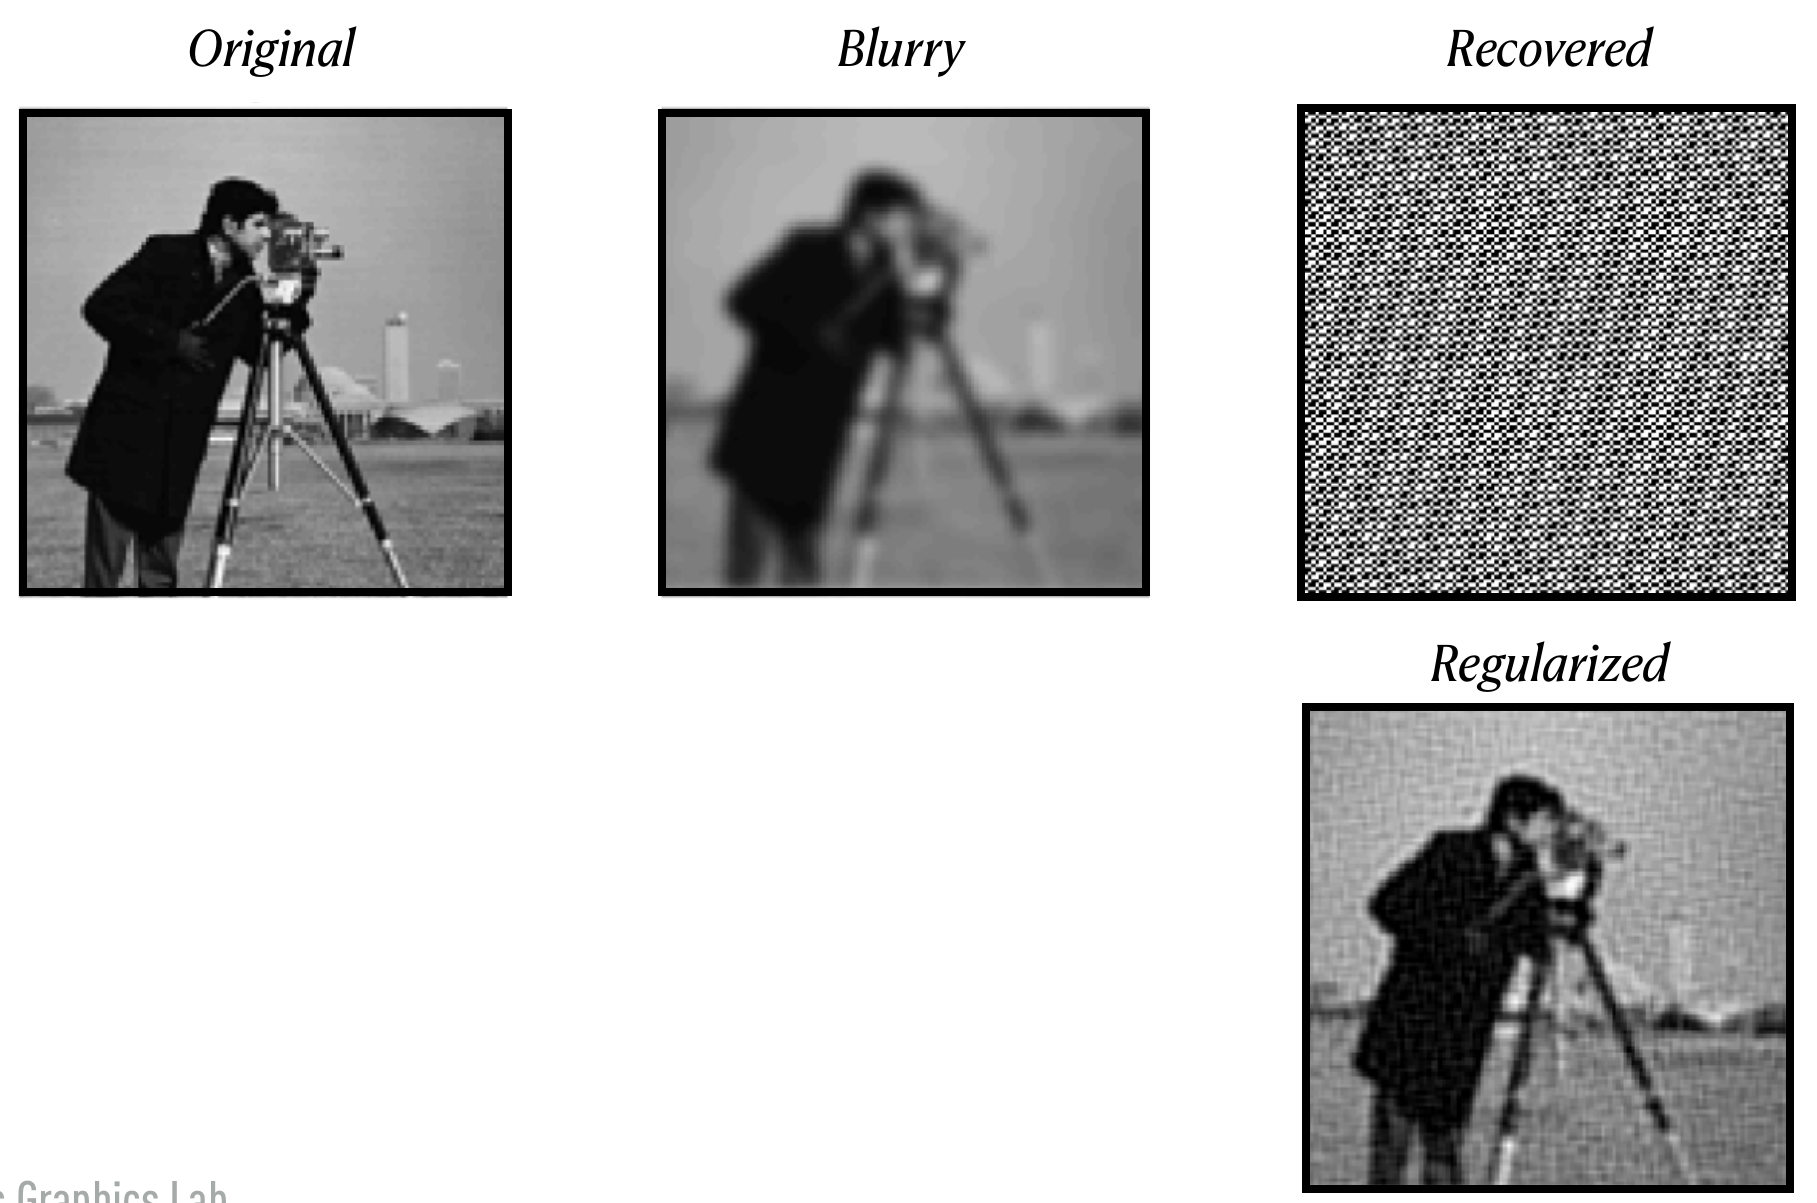
\includegraphics[
width=0.85\linewidth
]{../images/week03_01.png}

\end{center}

\end{example}



%=========================================================
\section{Forward and Backward Error of Solvers}


\begin{important}

Recap: backward error in the input space, forward error in the output space.

\[
\text{Condition number: ratio } \frac{\text{forward error}}{\text{backward error}}
\]

\end{important}


\begin{formula}

\textbf{Applied to linear system solving}

\begin{itemize}

\item Theoretical infinite precision solver:
$\mathbf{x} = f(\mathbf{b}) = \mathbf{A}^{-1}\mathbf{b}$. Its inverse is simple:
$f^{-1}(\mathbf{x}) = \mathbf{A}\mathbf{x}$.

\item Actual finite precision solver: $\hat{\mathbf{x}} = \hat{f}(\mathbf{b})$ -- how accurate is
$\hat{\mathbf{x}}$? Natural to expect
$f^{-1}(\hat{\mathbf{x}}) = \mathbf{A}\hat{\mathbf{x}} \approx \mathbf{b}$.

\end{itemize}

\end{formula}


\begin{definition}

\textbf{RESIDUAL}

\[
r(\hat{\mathbf{x}}) = \mathbf{A}\hat{\mathbf{x}} - \mathbf{b}
\]

Gives an approximation of the \textbf{backward error} of a linear system solver.

\end{definition}



%=========================================================
\section{The Matrix Norm}


Interlude: a matrix maps the points of a circle to an ellipse (an ellipsoid in higher
dimensions).


\begin{definition}

\textbf{MATRIX NORM} (aka.\ operator norm)

\[
\|\mathbf{A}\| = \max\{\|\mathbf{A}\mathbf{x}\|, \text{ where } \|\mathbf{x}\| = 1\}
\]

Determines the maximum radius of the ellipse that $\mathbf{A}$ makes of the unit circle.

\end{definition}


\begin{formula}

\textbf{Some inequalities}

\[
\|\mathbf{A}\mathbf{x}\| \le \|\mathbf{A}\|\,\|\mathbf{x}\|
\]

The length of a transformed vector is bounded by its original length and the most that it can
be stretched by $\mathbf{A}$.

\[
\|\mathbf{A}\mathbf{B}\| \le \|\mathbf{A}\|\,\|\mathbf{B}\|
\]

Successive application of $\mathbf{A}$ and $\mathbf{B}$ cannot stretch a vector by more than the
product of their individual bounds.

\end{formula}



%=========================================================
\section{Condition Number of a Linear System}


\begin{formula}

\textbf{Solving a perturbed linear system}

\begin{itemize}

\item Original system: $\mathbf{A}\mathbf{x} = \mathbf{b}$

\item Perturbed system: $\mathbf{A}(\mathbf{x} + \Delta\mathbf{x}) = \mathbf{b} +
\Delta\mathbf{b}$

\item What we'd like to know: how big is $\|\Delta\mathbf{x}\| / \|\mathbf{x}\|$ (relative error
of the solution)?

\end{itemize}

\textbf{Ingredient 1}:
$\|\mathbf{b}\| = \|\mathbf{A}\mathbf{x}\| \le \|\mathbf{A}\| \cdot \|\mathbf{x}\|
\Leftrightarrow \|\mathbf{x}\| \ge \frac{\|\mathbf{b}\|}{\|\mathbf{A}\|}$

\textbf{Ingredient 2}:
$\|\Delta\mathbf{x}\| = \|\mathbf{A}^{-1}\Delta\mathbf{b}\| \le \|\mathbf{A}^{-1}\| \cdot
\|\Delta\mathbf{b}\|$

\textbf{Putting it together}:

\[
\frac{\|\Delta\mathbf{x}\|}{\|\mathbf{x}\|}
\le \underbrace{\|\mathbf{A}^{-1}\| \cdot \|\mathbf{A}\|}_{= \operatorname{cond}(\mathbf{A})
= \kappa(\mathbf{A})} \cdot \frac{\|\Delta\mathbf{b}\|}{\|\mathbf{b}\|}
\]

\end{formula}


\begin{definition}

\textbf{CONDITION NUMBER}

\[
\operatorname{cond}(\mathbf{A}) = \|\mathbf{A}\| \cdot \|\mathbf{A}^{-1}\|
\]

Measures how much $\mathbf{A}$ (and $\mathbf{A}^{-1}$) distort the unit circle: the more
elongated the ellipse, the larger the condition number.

\end{definition}


\begin{center}

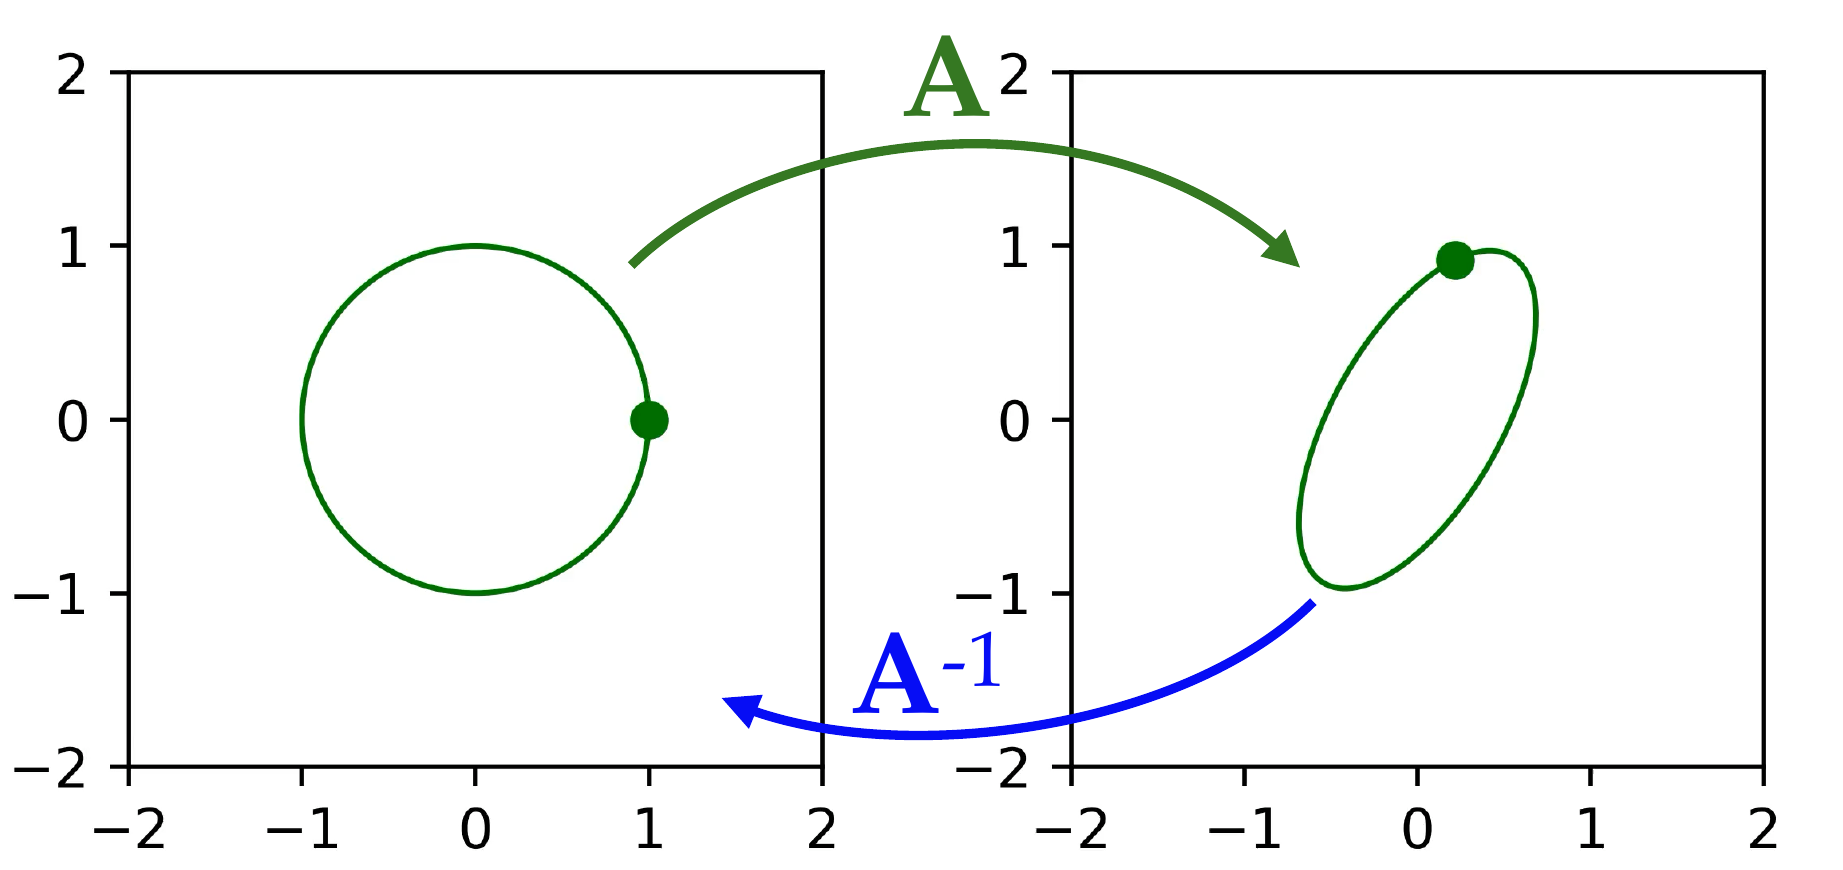
\includegraphics[
width=0.85\linewidth
]{../images/week03_02.png}

\end{center}



%=========================================================
\section{Properties of the Condition Number}


\begin{summary}

\begin{itemize}

\item $\operatorname{cond}(\mathbf{A}) = \infty$ iff $\mathbf{A}$ is singular

\item $\operatorname{cond}(\mathbf{A}) = 1$ if $\mathbf{A}$ is the identity matrix

\item $\operatorname{cond}(\gamma\mathbf{A}) = \operatorname{cond}(\mathbf{A})$,
$\gamma \in \mathbb{R}$

\item $\operatorname{cond}(\mathbf{Q}\mathbf{A}) = \operatorname{cond}(\mathbf{A})$ where
$\mathbf{Q}$ is a rotation matrix

\end{itemize}

\end{summary}


\begin{warning}

\textbf{What about the determinant?} It is \emph{not} a good way to determine whether a linear
system is easy to solve. We know that $\det(\mathbf{A}) = 0$ iff $\mathbf{A}$ is singular. But
with $\mathbf{A} = \frac{1}{10}\mathbf{I} \in \mathbb{R}^{1000 \times 1000}$,
$\det(\mathbf{A}) = 10^{-1000}$, yet this linear system is \emph{trivial} to solve. On the other
hand, $\operatorname{cond}(\mathbf{A}) = 1$ (!)

\end{warning}


\begin{important}

\textbf{Implications} (stated without proof): if you are using a good linear system solver, and
if $\mathbf{b}$ can be assumed to be accurate, then

\[
\frac{\|\Delta\mathbf{x}\|}{\|\mathbf{x}\|} \lesssim \operatorname{cond}(\mathbf{A})\,
\operatorname{ulp}(1)
\]

where $\operatorname{ulp}(1) \approx 2^{-23}$ (single precision), $\approx 2^{-52}$ (double
precision).

\end{important}


\begin{warning}

\textbf{A chicken-and-egg problem}: inverting matrices is expensive; we want to know the
condition number to find out if this is even possible\dots\ but our definition of
$\operatorname{cond}(\mathbf{A})$ requires inverting a matrix and computing a matrix norm (how?!).
Stay tuned!

\end{warning}



%=========================================================
\section{Badly Conditioned Systems}


\begin{important}

\textbf{Geometry} (row-based interpretation): noise \& errors may be greatly magnified. When the
planes (lines) $\mathbf{a}^{(i)} \cdot \mathbf{x} = b_i$ are nearly parallel, a small uncertainty
on each one gives a huge region of possible intersections.

\end{important}


\begin{center}

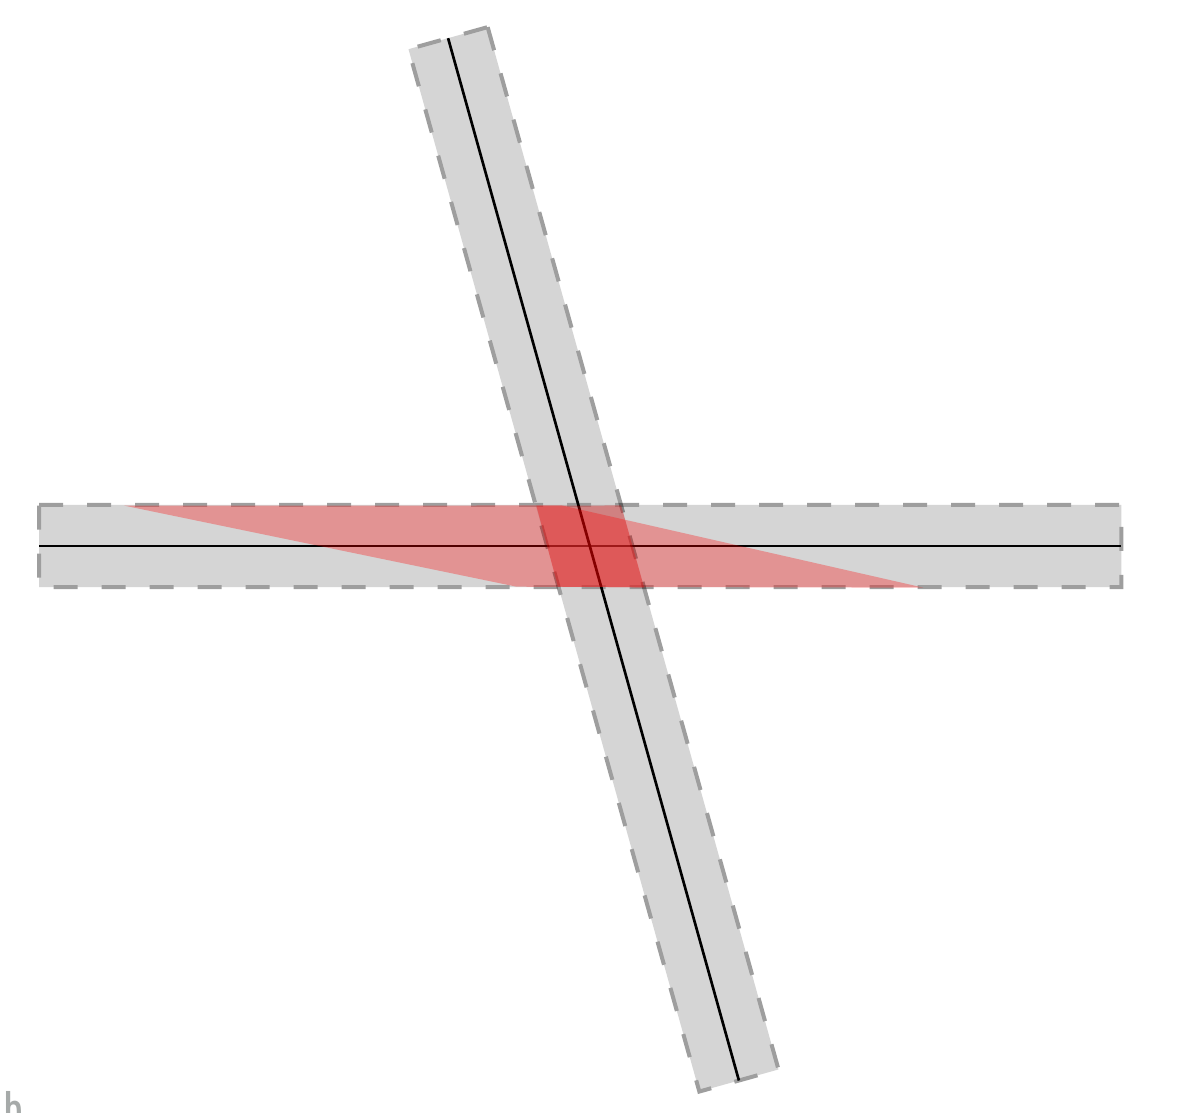
\includegraphics[
width=0.6\linewidth
]{../images/week03_03.png}

\end{center}


\begin{example}

\textbf{Conditioning of the Vandermonde matrix} (maps polynomial coefficients to polynomial
evaluations):

\[
\mathbf{A} = \begin{pmatrix}
\alpha_1^n & \dots & \alpha_1^2 & \alpha_1 & 1 \\
\vdots & & \vdots & \vdots & \vdots \\
\alpha_m^n & \dots & \alpha_m^2 & \alpha_m & 1
\end{pmatrix}
\]

Condition number for $n = 100$ (uniformly spaced positions on $[0, 1]$):

\[
\operatorname{cond}(\mathbf{A}) = 7.31 \cdot 10^{19} \ (!!!!!!)
\]

\end{example}



%=========================================================
\section{Linear Least Squares}


\begin{definition}

\textbf{FROM LINEAR SYSTEMS TO LEAST SQUARES}

$n$ constraint equations (many), $m$ parameters (few): instead of
$\mathbf{A}\mathbf{x} = \mathbf{b}$, ask for
$\|\mathbf{A}\mathbf{x} - \mathbf{b}\| \approx 0$. For almost all values of $\mathbf{b}$, this
\emph{tall} system is not solvable (generally ill-defined): try to get as close as possible.

\end{definition}


\begin{formula}

\textbf{Compromise: minimize the residual}
$\|\mathbf{r}(\mathbf{x})\| = \|\mathbf{A}\mathbf{x} - \mathbf{b}\|$.

\textbf{1. Expand} (the squared length of a vector is the inner product with itself):

\begin{align*}
\|\mathbf{A}\mathbf{x} - \mathbf{b}\|^2
&= \langle \mathbf{A}\mathbf{x} - \mathbf{b}, \mathbf{A}\mathbf{x} - \mathbf{b} \rangle \\
&= \langle \mathbf{A}\mathbf{x}, \mathbf{A}\mathbf{x} \rangle
- \langle \mathbf{A}\mathbf{x}, \mathbf{b} \rangle
- \langle \mathbf{b}, \mathbf{A}\mathbf{x} \rangle
+ \langle \mathbf{b}, \mathbf{b} \rangle \\
&= \mathbf{x}^T\mathbf{A}^T\mathbf{A}\mathbf{x} - 2\mathbf{b}^T\mathbf{A}\mathbf{x}
+ \|\mathbf{b}\|^2
\end{align*}

\textbf{2. Take the derivative} ($\|\mathbf{b}\|^2$ is constant):

\[
\frac{\partial}{\partial\mathbf{x}}\left[\mathbf{x}^T\mathbf{A}^T\mathbf{A}\mathbf{x}
- 2\mathbf{b}^T\mathbf{A}\mathbf{x} + \|\mathbf{b}\|^2\right]
= 2\mathbf{A}^T\mathbf{A}\mathbf{x} - 2\mathbf{A}^T\mathbf{b}
\]

\textbf{3. Set it to zero} (Carl Friedrich Gauss):

\[
\mathbf{A}^T\mathbf{A}\mathbf{x} = \mathbf{A}^T\mathbf{b}
\qquad \text{(\textbf{normal equations})}
\]

\end{formula}


\begin{important}

The ``best'' solution (in the $L_2$ sense) is given by the normal equations, which are
equivalent to a \textbf{smaller square linear system} ($\mathbf{A}^T\mathbf{A}$ is
$m \times m$).

\end{important}


\begin{definition}

\textbf{WHY ``NORMAL'' EQUATIONS?}

$\mathbf{A}^T(\mathbf{A}\mathbf{x} - \mathbf{b}) = \mathbf{0}$: at the optimum, the residual
$\mathbf{r}(\mathbf{x})$ is \textbf{normal} (perpendicular) to $\operatorname{span}(\mathbf{A})$;
$\mathbf{y} = \mathbf{A}\mathbf{x}$ is the orthogonal projection of $\mathbf{b}$.

\end{definition}


\begin{center}

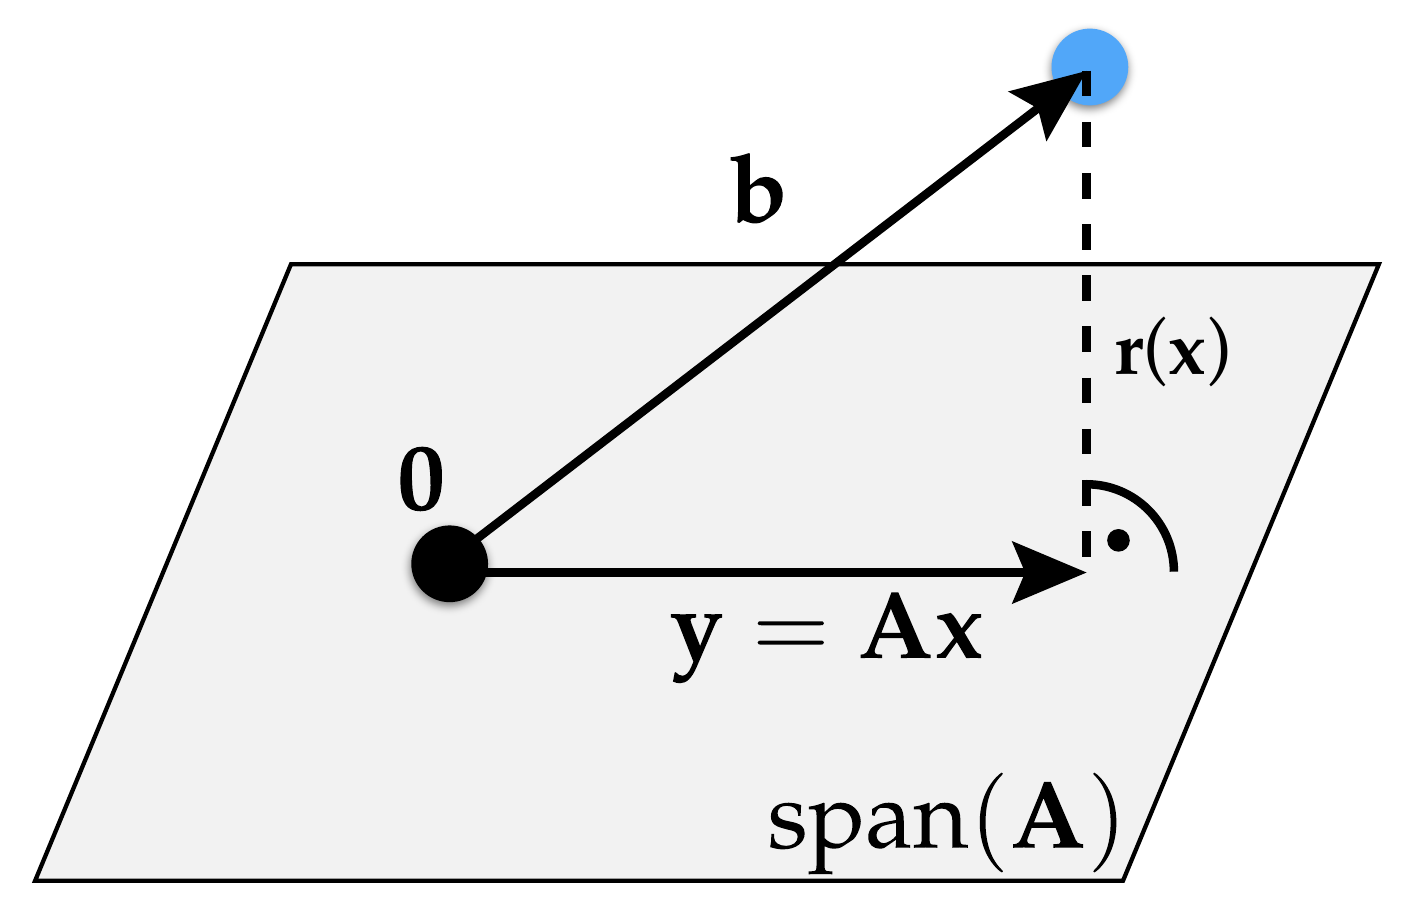
\includegraphics[
width=0.6\linewidth
]{../images/week03_04.png}

\end{center}



%=========================================================
\section{Weekly Summary}


\begin{summary}

\begin{itemize}

\item Pick the solver for the matrix type; factorization $\mathcal{O}(n^3)$, substitution
$\mathcal{O}(n^2)$.

\item Regression: data + model linear in the unknowns $\Rightarrow$ linear system (Vandermonde
matrix for polynomials).

\item Residual $\mathbf{A}\hat{\mathbf{x}} - \mathbf{b}$ $\approx$ backward error.

\item Matrix norm, $\operatorname{cond}(\mathbf{A}) = \|\mathbf{A}\|\,\|\mathbf{A}^{-1}\|$,
relative error $\lesssim \operatorname{cond}(\mathbf{A})\operatorname{ulp}(1)$; the determinant
says nothing about difficulty.

\item Least squares: minimize $\|\mathbf{A}\mathbf{x} - \mathbf{b}\|^2$ $\Rightarrow$ normal
equations $\mathbf{A}^T\mathbf{A}\mathbf{x} = \mathbf{A}^T\mathbf{b}$.

\end{itemize}

\end{summary}



\end{multicols}


\end{document}
